\section{Cooling and Mixing}

\boxit{Newton's Law of Cooling}

\noindent
Newton's law of cooling states that if an object with temperature
$T(t)$ at time $t$ is in a medium with temperature $T_m(t)$,  the
rate of change of $T$ at time $t$ is proportional to $T(t)-T_m(t)$;
thus,
$T$ satisfies a differential equation of the form
\begin{equation} \label{eq:4.2.1}
T'=-k(T-T_m).
\end{equation}
 Here $k > 0$, since the temperature of the object must decrease if
$T > T_m$, or increase if $T < T_m$.  We'll call $k$  the {\color{blue}\it
temperature decay constant of the medium\/}.

For simplicity, in this section we'll assume  that the medium is
maintained at a constant temperature $T_m$. This is another example of
 building a simple mathematical model for a physical
phenomenon. Like most mathematical models it has its limitations. For
example, it's reasonable to assume that the temperature of a room
remains approximately constant if the cooling object is a cup of
coffee, but perhaps not if it's a huge cauldron of molten metal. (For
more on this see Exercise~\ref{exer:4.2.17}.)

To solve  \eqref{eq:4.2.1}, we rewrite it as
$$
T'+kT=kT_m.
$$
Since $e^{-kt}$ is a solution of the complementary equation, the
solutions of this equation are of the form $T=ue^{-kt}$, where
$u'e^{-kt}=kT_m$, so $u'=kT_me^{kt}$. Hence,
$$
u=T_me^{kt}+c,
$$
so
$$
T=ue^{-kt}=T_m+ce^{-kt}.
$$
If $T(0)=T_0$,  setting $t=0$ here yields $c=T_0-T_m$, so
\begin{equation} \label{eq:4.2.2}
T=T_m+(T_0-T_m)e^{-kt}.
\end{equation}
Note that $T-T_m$ decays exponentially, with decay constant $k$.

\begin{example}\label{example:4.2.1}\rm
A ceramic insulator is baked at $400^\circ$C and cooled in a room in
which the temperature is $25^\circ$C. After 4 minutes the
temperature of the insulator is $200^\circ$C. What is its temperature
after 8 minutes?
\end{example}

\solution Here $T_0=400$ and $T_m=25$, so \eqref{eq:4.2.2} becomes
\begin{equation} \label{eq:4.2.3}
T=25+375e^{-kt}.
\end{equation}
 We determine $k$ from the stated condition that  $T(4)=200$;
that is,
$$
200=25+375e^{-4k};
$$
 hence,
$$
e^{-4k} = {175\over 375} = {7\over 15}.
$$
 Taking logarithms and solving for $k$ yields
$$
k=-{1\over 4} \ln {7\over 15}={1\over 4}\ln {15\over 7}.
$$
 Substituting this into \eqref{eq:4.2.3} yields
$$
T=25+375 e^{-{t\over 4} \ln {15\over 7}}
$$
(Figure~\ref{figure:4.2.1}).
Therefore the temperature of the insulator after
8 minutes is
$$\begin{array}{rl}
T(8) & \dst = 25+375 e^{-2 \ln {15\over 7}} \\[9pt]
& \dst = 25+375 \left({7\over 15}\right)^2 \approx
107^\circ \mbox{C}.
\end{array}$$

\begin{figure}[tbp]
  \centering
  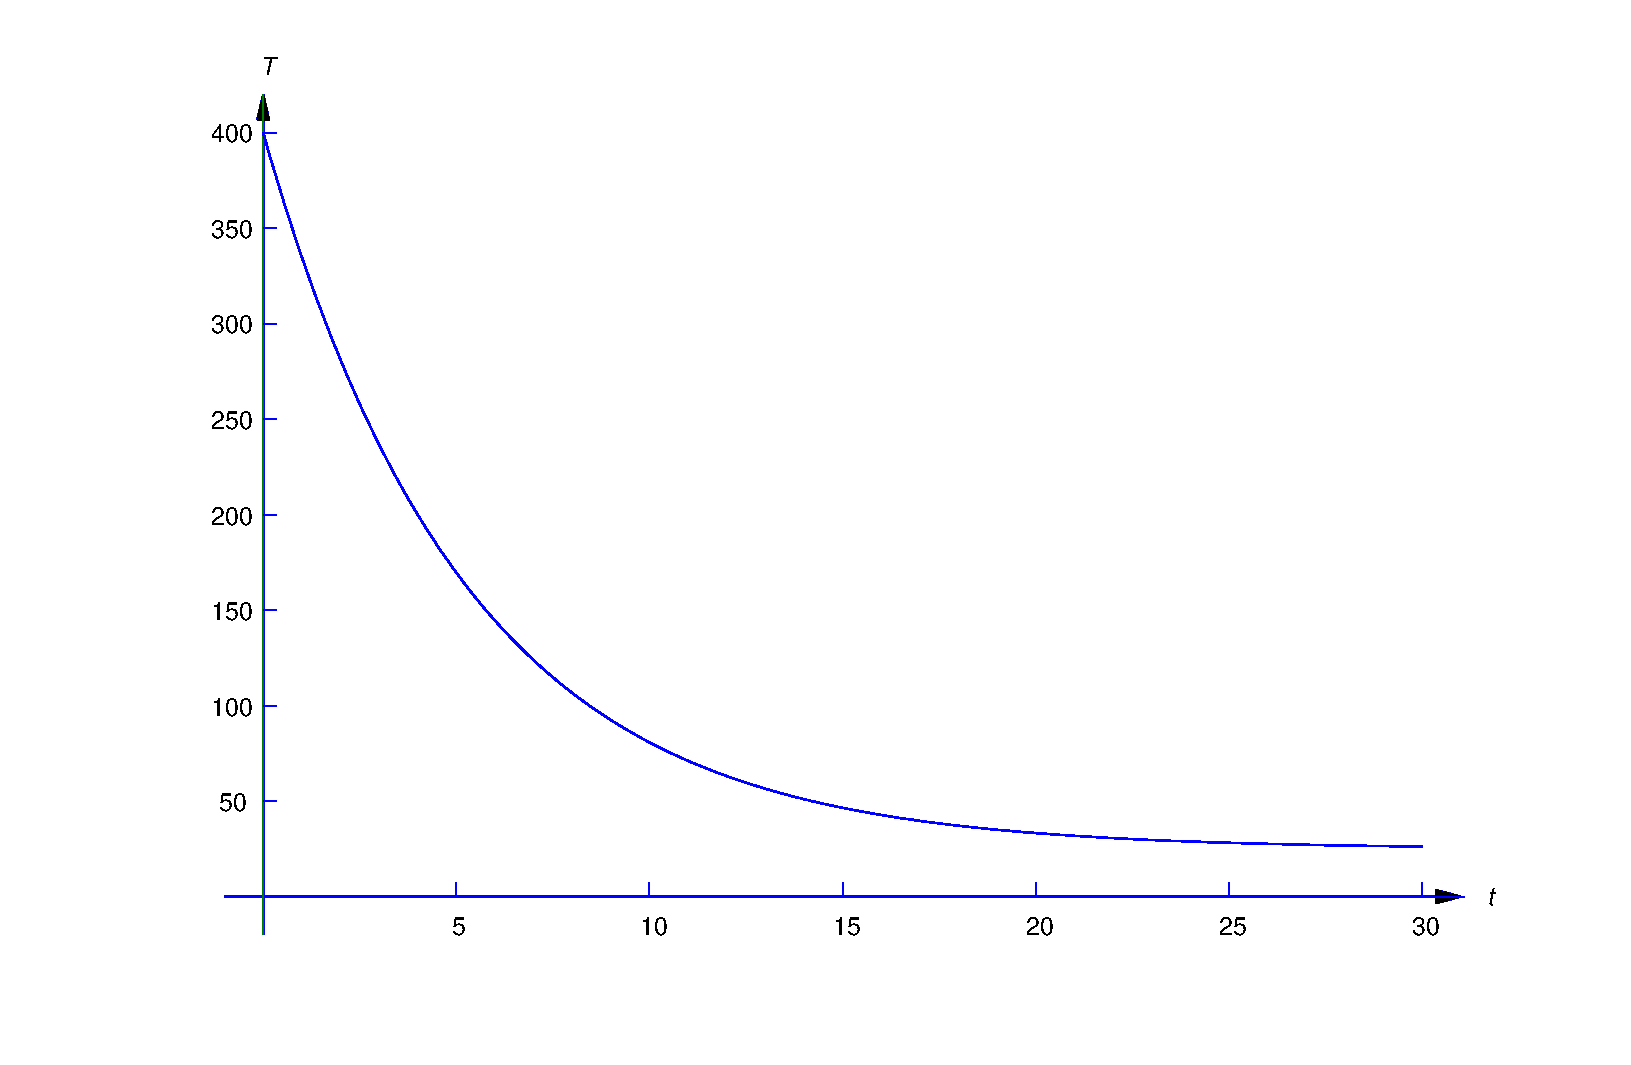
\includegraphics[bb=-78 148 689 643,width=5.67in,height=3.66in,keepaspectratio]{fig040201}
\color{blue}
\caption{$T=25+375e^{-(t/4)\ln 15/7}$}
  \label{figure:4.2.1}
\end{figure}

\begin{example}\label{example:4.2.2}\rm
An object with temperature $72^\circ$F is placed outside, where the
temperature is $-20^\circ$F. At 11:05 the temperature of the object
is $60^\circ$F and at 11:07 its temperature is $50^\circ$F. At what
time was the object placed outside?
\end{example}

\solution Let $T(t)$ be the temperature of the object at time $t$. For
convenience, we choose the origin $t_0=0$ of the time scale to be
11:05 so that $T_0=60$. We must determine the time $\tau$ when
$T(\tau)=72$. Substituting $T_0=60$ and $T_m=-20$ into \eqref{eq:4.2.2}
yields
$$
T  = -20+\bigl(60-(-20)\bigr)e^{-kt}
$$
 or
\begin{equation} \label{eq:4.2.4}
T = -20+80e^{-kt}.
\end{equation}
We obtain $k$ from the stated condition that the temperature of the
object is 50$^\circ$F at 11:07. Since 11:07 is $t=2$ on our time
scale, we can determine $k$ by substituting $T=50$ and $t=2$ into
\eqref{eq:4.2.4} to obtain
$$
50 = -20+80e^{-2k}
$$
(Figure~\ref{figure:4.2.2});
 hence,
$$
e^{-2k}={70\over 80}={7\over 8}.
$$
 Taking logarithms and solving for $k$ yields
$$
k =-{1\over 2} \ln {7\over 8} = {1\over 2} \ln {8\over 7}.
$$
 Substituting this into \eqref{eq:4.2.4} yields
$$
T = -20+80 e^{-{t\over 2}\ln {8\over 7}},
$$
 and the condition $T(\tau)=72$  implies that
$$
72 =-20+80 e^{-{\tau\over 2} \ln {8\over 7}};
$$
 hence,
$$
e^{-{\tau\over 2} \ln {8\over 7}} ={92\over 80} =
{23\over 20}.
$$
Taking logarithms and solving for $\tau$ yields
$$
\tau = -{2 \ln {23\over 20}\over \ln {8\over 7}} \approx-2.09\
\mbox{min}.
$$
Therefore the object was placed outside
about 2 minutes and 5 seconds before 11:05; that is,
at 11:02:55.

\begin{figure}[tbp]
  \centering
  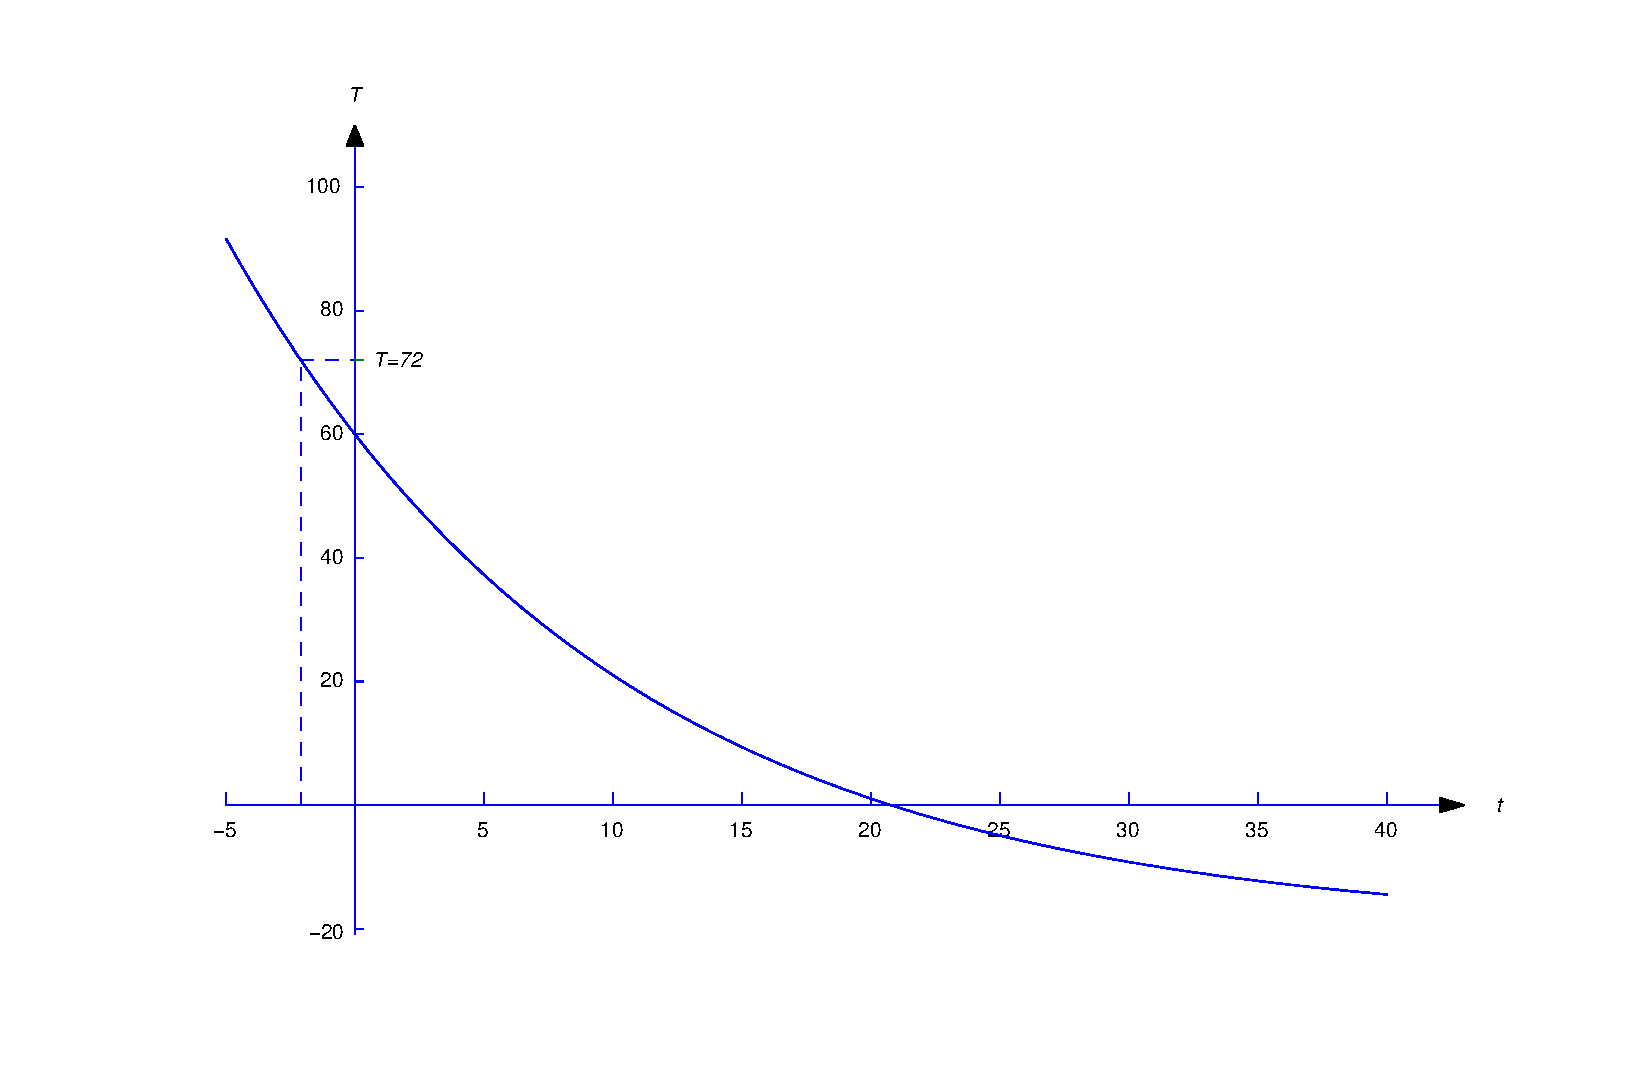
\includegraphics[bb=-78 148 689 643,width=5.67in,height=3.66in,keepaspectratio]{fig040202}
\color{blue}
  \caption{$T = -20+80 e^{-{t\over 2}\ln {8\over 7}}$}
  \label{figure:4.2.2}
\end{figure}

\boxit{Mixing Problems}

\noindent
In the next two examples a saltwater solution with a given
concentration (weight of salt per unit volume of solution) is added at
a specified rate to a tank that initially contains saltwater with a
different concentration. The problem is to determine the quantity of
salt in the tank as a function of time. This is an example of a {\color{blue}\it
mixing problem\/}. To construct a tractable mathematical model for
mixing problems we assume in our examples (and most exercises) that
the mixture is stirred instantly so that the salt is always uniformly
distributed throughout the mixture. Exercises~\ref{exer:4.2.22}
and \ref{exer:4.2.23} deal with situations where this isn't  so, but
the distribution of salt becomes approximately uniform as
$t\to\infty$.

\begin{example}\label{example:4.2.3}  \rm
A tank initially contains 40 pounds of salt dissolved in 600 gallons
of water. Starting at $t_0 = 0$, water that contains 1/2 pound of salt
per gallon is poured into the tank at the rate of 4 gal/min and the
mixture is drained from the tank at the same rate
(Figure~\ref{figure:4.2.3}).
\begin{alist}
\item % (a)
Find a differential equation for the quantity $Q(t)$ of salt in the
tank at time $t > 0$, and solve the equation to determine $Q(t)$.
\item % (b)
 Find $\lim_{t\to\infty}Q(t)$.
\end{alist}
\end{example}

\begin{figure}[tbp]
  \centering
  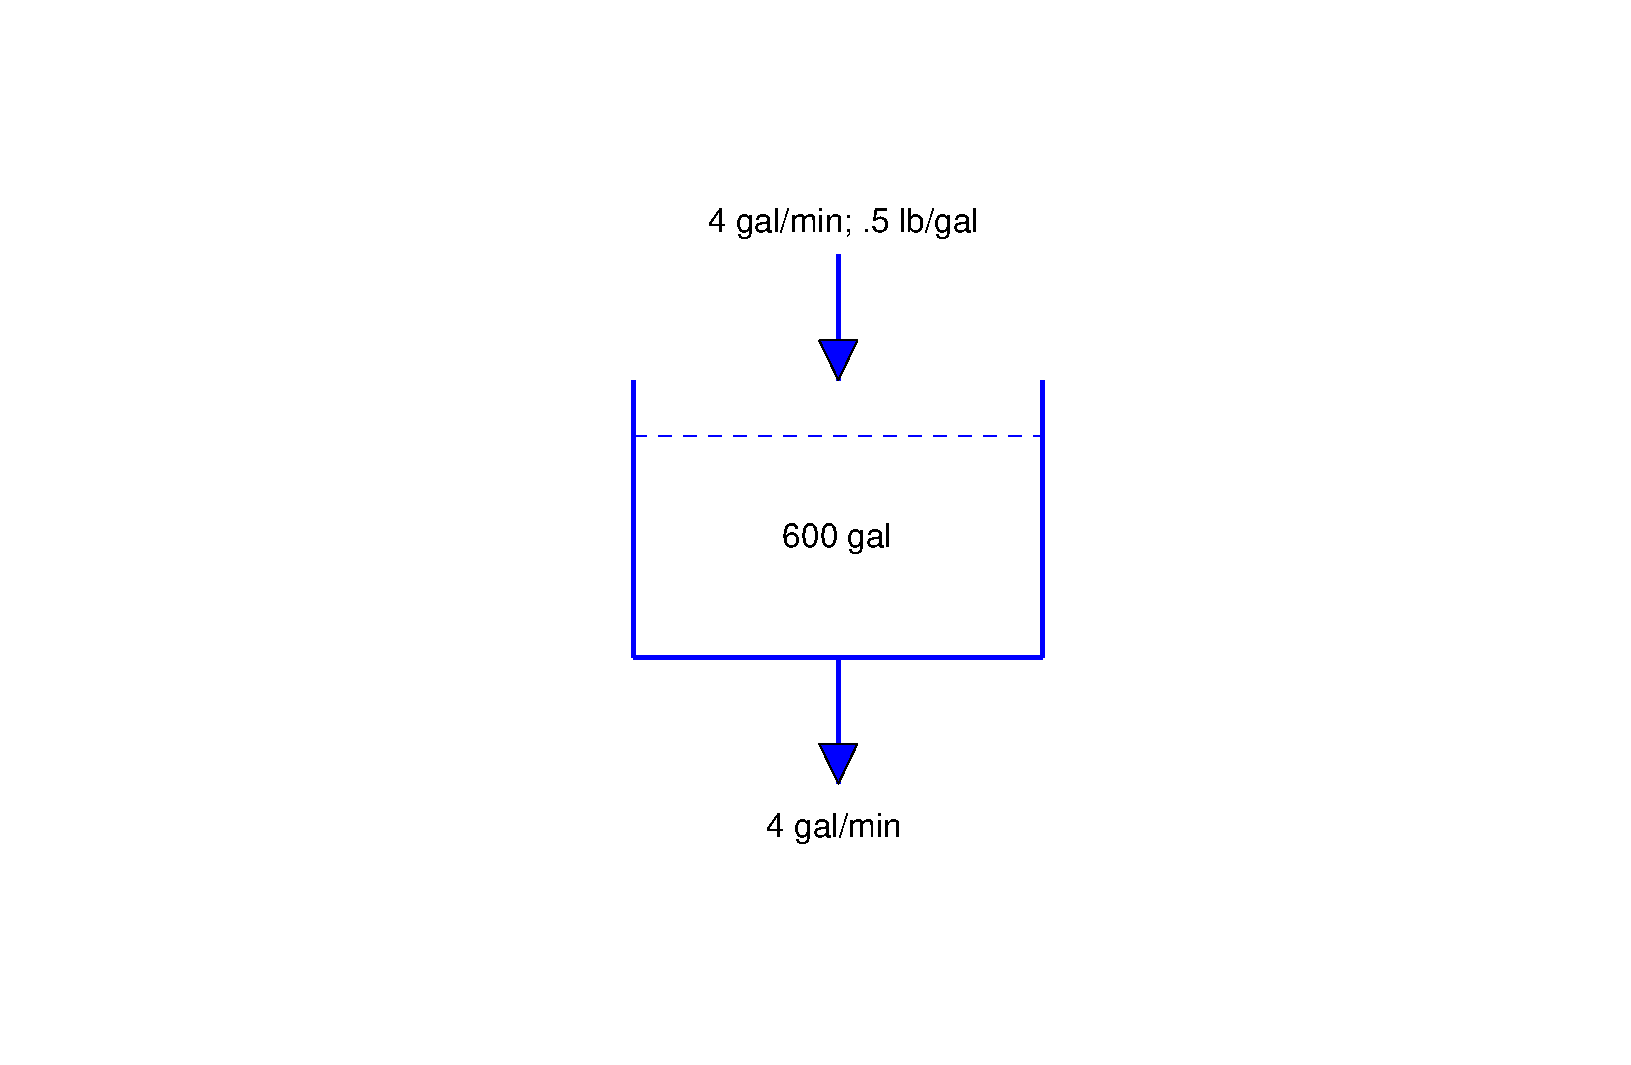
\includegraphics[bb=-78 148 689 643,width=5.67in,height=3.66in,keepaspectratio]{fig040203}
\color{blue}
  \caption{A mixing problem}
  \label{figure:4.2.3}
\end{figure}

\solutionpart{a} To find a differential equation for $Q$, we must use
the given information to derive an expression for $Q'$. But $Q'$
is the rate of change of the quantity of salt in the tank changes with
respect to time;
  thus, if {\color{blue}\it rate in\/} denotes the rate at which
salt enters
the tank and {\color{blue}\it rate out\/} denotes the rate by which it
leaves, then
\begin{equation} \label{eq:4.2.5}
Q' = \mbox{rate in}-\mbox{rate out}.
\end{equation}
The rate in is
$$
\left({1\over 2}\  \mbox{lb/gal}\right) \times (4\  \mbox{gal/min}) = 2\
\mbox{lb/min}.
$$
Determining the rate out requires a little more thought. We're
removing 4 gallons of the mixture per minute, and there are always 600
gallons in the tank; that is, we're removing $1/150$ of the mixture
per minute. Since the salt is evenly distributed in the mixture, we
are also removing $1/150$ of the salt per minute. Therefore, if there
are $Q(t)$ pounds of salt in the tank at time $t$, the rate out
at any time $t$ is $Q(t)/150$. Alternatively, we can arrive at this
conclusion by arguing that
$$
\begin{array}{lcl}
\mbox{rate out} & = & (\mbox{concentration})\times(\mbox{rate of
flow out})\\[6pt] \mbox{}&=&(\mbox{lb/gal})\times(\mbox{gal/min})\\[10pt]
&=&\dst{Q(t)\over600}\times
4=\dst{Q(t)\over150}.
\end{array}
$$
 We can now
write \eqref{eq:4.2.5} as
$$
Q' = 2-{Q\over 150}.
$$
This first order equation can be rewritten as
$$
Q'+{Q\over 150} = 2.
$$
Since $e^{-t/150}$ is a solution of the complementary equation, the
solutions of this equation are of the form  $Q=ue^{-t/150}$, where
$u'e^{-t/150}=2$, so $u'=2e^{t/150}$. Hence,
$$
u = 300e^{t/150}+c,
$$
 so
\begin{equation} \label{eq:4.2.6}
Q=ue^{-t/150}=300+ce^{-t/150}
\end{equation}
(Figure~\ref{figure:4.2.4}).
 Since $Q(0)=40$,  $c=-260$;  therefore,
$$
Q=300-260e^{-t/150}.
$$

\solutionpart{b} From \eqref{eq:4.2.6}, we see that that $\lim_{t \to
\infty}Q(t)=300$ for any value of  $Q(0)$. This is
intuitively reasonable, since the incoming solution contains 1/2
pound of salt per gallon and there are always 600 gallons of water in
the tank. \quad

\begin{example}\label{example:4.2.4} \rm
A 500-liter tank initially contains 10 g of salt dissolved in 200
liters of water. Starting at $t_0=0$, water that contains 1/4 g of salt
per liter is poured into the tank at the rate of 4 liters/min and the
mixture is drained from the tank at the rate of 2 liters/min
(Figure~\ref{figure:4.2.5}). Find a
differential equation for the quantity $Q(t)$ of salt in the tank at
time $t$ prior to the time when the tank overflows and find the
concentration $K(t)$ (g/liter ) of salt in the tank at any such time.
\end{example}

\begin{figure}[tbp]
  \centering
  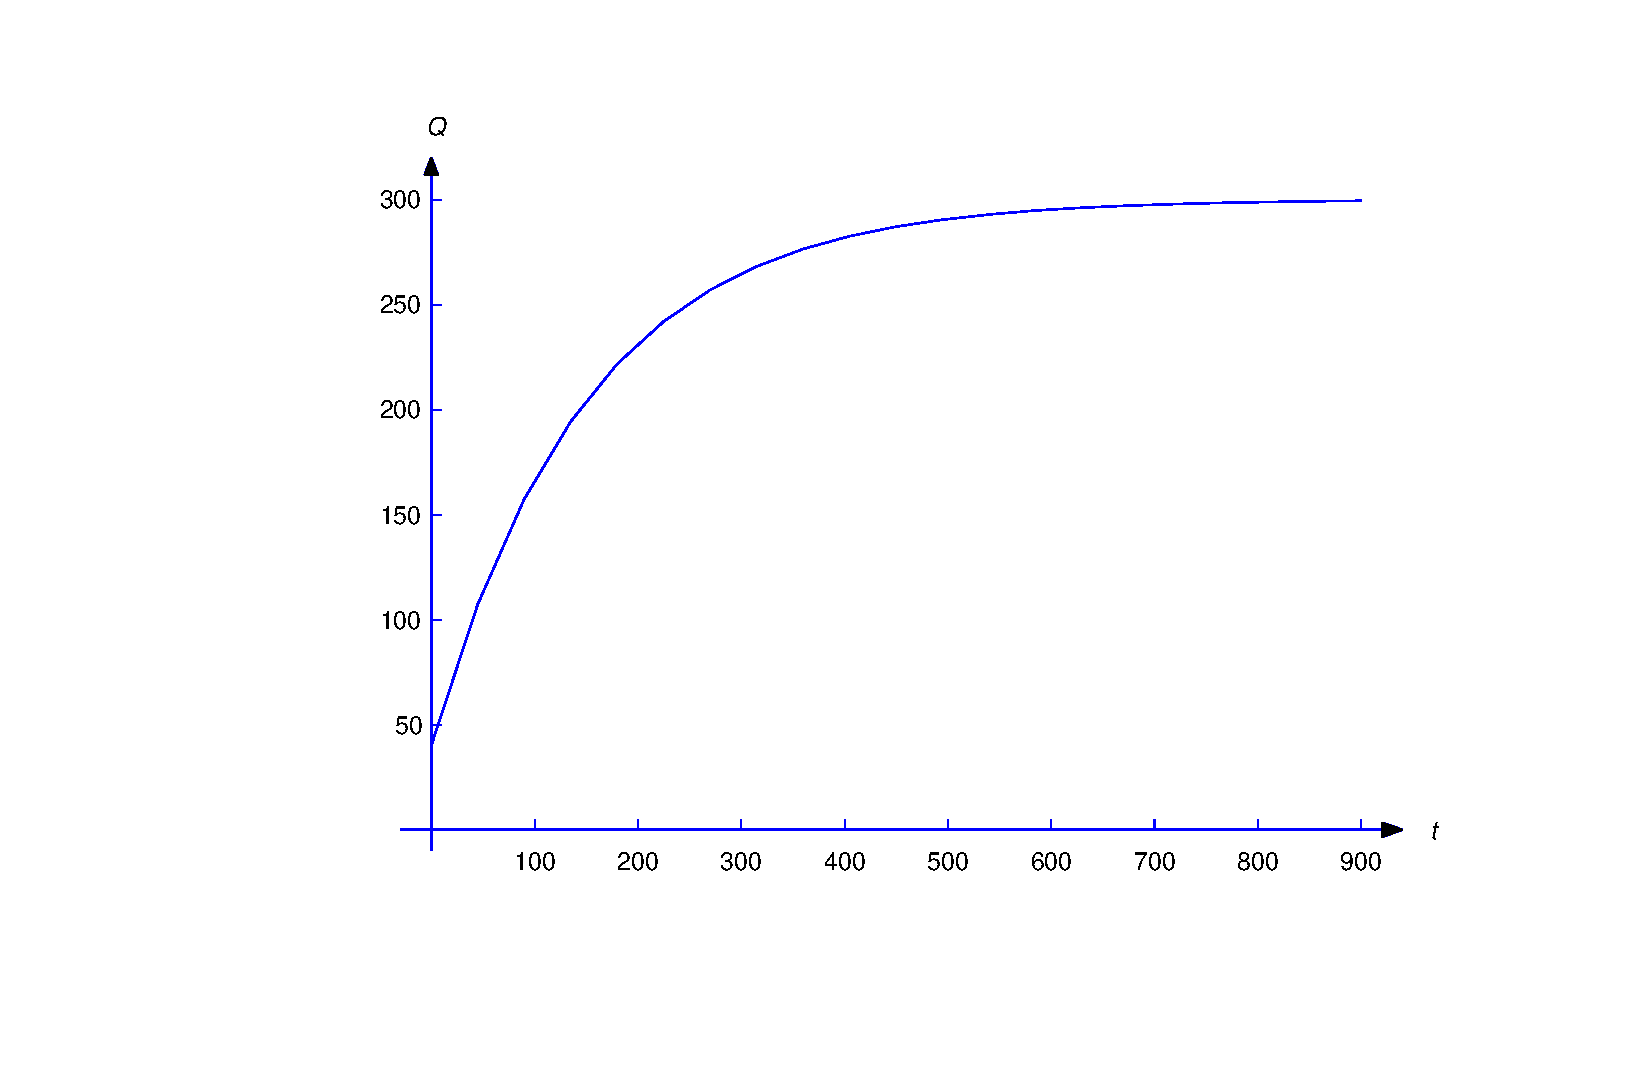
\includegraphics[bb=-78 148 689 643,width=5.67in,height=3.66in,keepaspectratio]{fig040204}
\color{blue}
  \caption{$Q=300-260e^{-t/150}$}
  \label{figure:4.2.4}
\end{figure}

\begin{figure}[tbp]
  \centering
  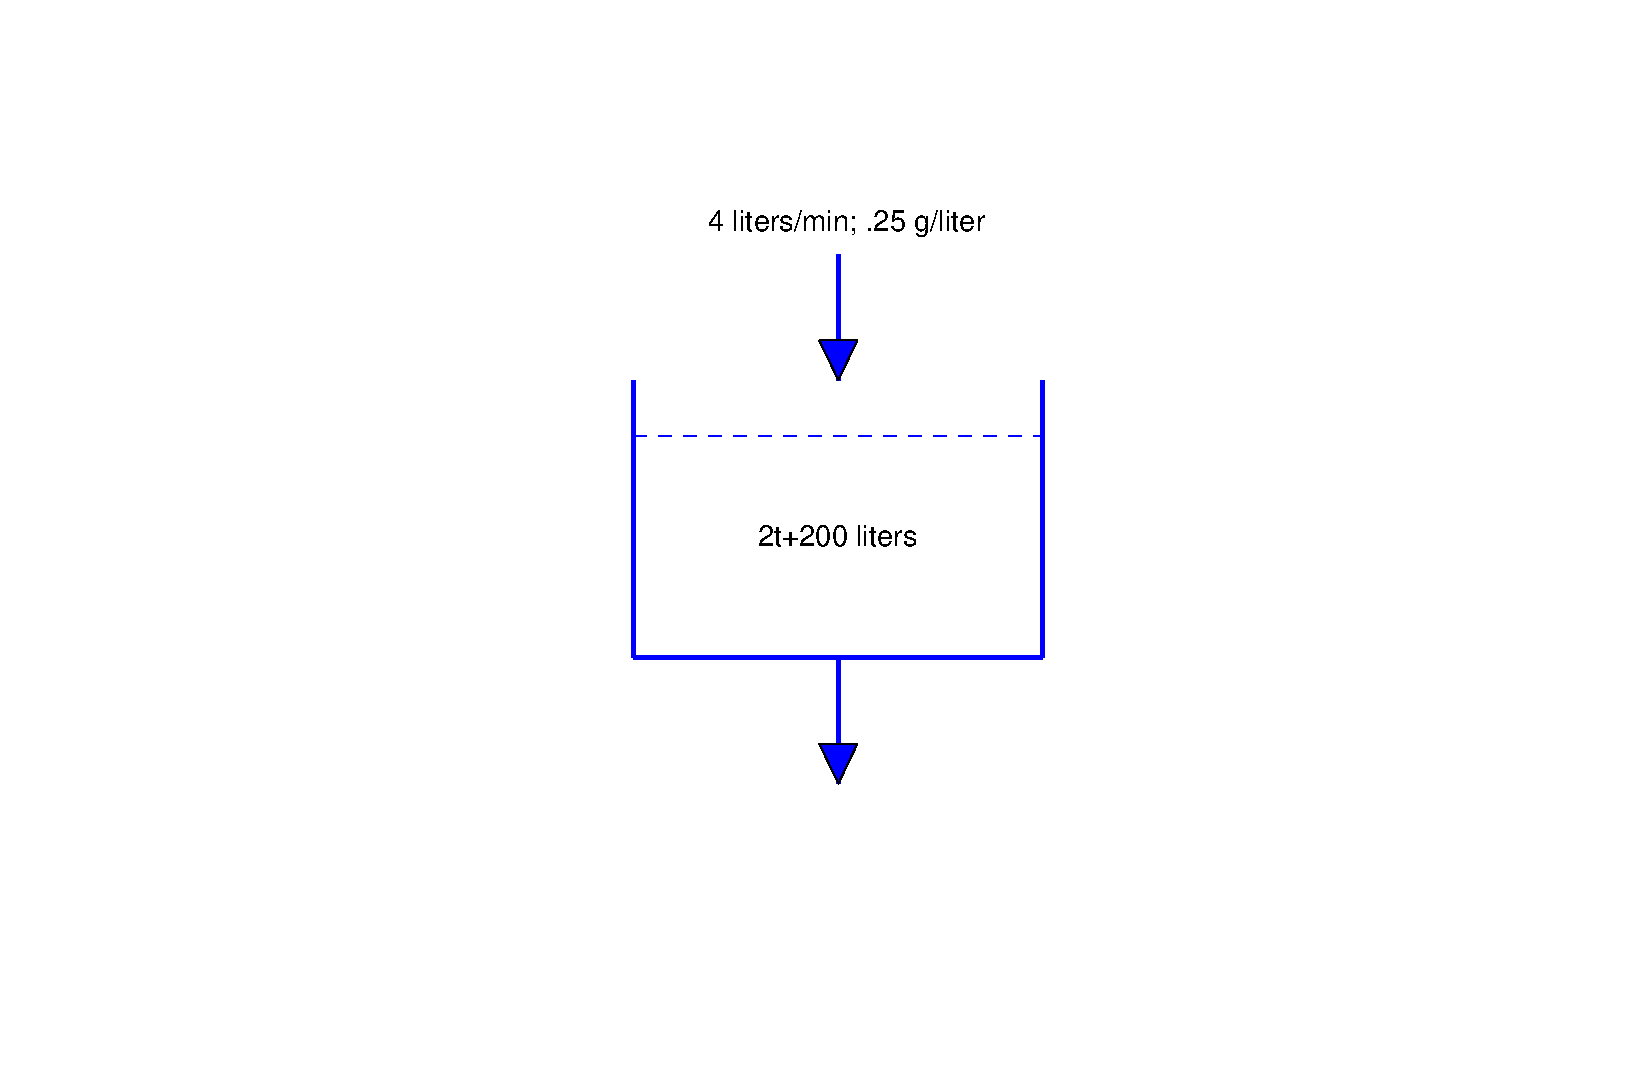
\includegraphics[bb=-78 148 689 643,width=5.67in,height=3.66in,keepaspectratio]{fig040205}
\color{blue}
  \caption{Another mixing problem}
  \label{figure:4.2.5}
\end{figure}

\solution  We first determine the
amount $W(t)$ of solution in the tank at any time $t$ prior to
overflow.  Since $W(0) = 200$ and we're adding 4 liters/min while
 removing only 2 liters/min, there's a net gain
of 2 liters/min in the tank;  therefore,
$$
W(t) = 2t+200.
$$
 Since $W(150)=500$ liters (capacity of the
tank), this formula is valid for $0 \le t \le 150$.

Now let $Q(t)$ be the number of grams of salt in the tank
at time $t$, where  $0 \le t \le 150$.  As in Example~\ref{example:4.2.3},
\begin{equation} \label{eq:4.2.7}
Q' = \mbox{rate in}-\mbox{rate out}.
\end{equation}
 The rate in is
\begin{equation} \label{eq:4.2.8}
\left({1\over 4}\  \mbox{g/liter}\,\right) \times (4\
\mbox{liters/min}\,) = 1\  \mbox{g/min}.
\end{equation}
 To determine the rate out, we observe that since
the mixture is being removed from the tank at the constant
rate of 2 liters/min and there are $2t+200$
liters in the tank at time $t$, the fraction of the mixture
being removed per minute at time $t$ is
$$
{2\over 2t+200} = {1\over t+100}.
$$
We're removing this same fraction of the salt per
minute.  Therefore, since there are $Q(t)$ grams of salt in
the tank at time $t$,
\begin{equation} \label{eq:4.2.9}
\mbox{rate out} = {Q(t)\over t+100}.
\end{equation}
Alternatively, we can arrive at this conclusion by arguing that
$$
\begin{array}{lcl}
\mbox{rate out} & = & (\mbox{concentration})\times(\mbox{rate of
flow out})
=(\mbox{g/liter})\times(\mbox{liters/min})\\[10pt]
&=&\dst{Q(t)\over2t+200}\times
2=\dst{Q(t)\over t+100}.
\end{array}
$$
 Substituting \eqref{eq:4.2.8} and \eqref{eq:4.2.9} into \eqref{eq:4.2.7}
yields
\begin{equation} \label{eq:4.2.10}
Q'=1-{Q\over t+100},\quad\text{ \rm so }\quad
Q'+{1\over t+100} Q=1.
\end{equation}
By separation of variables, $1/(t+100)$ is a solution of the
complementary equation, so the solutions of \eqref{eq:4.2.10}
are of the form
$$
Q={u\over t+100},\mbox{\quad where \quad}{u'\over t+100}=1,\mbox{\quad
so \quad} u'=t+100.
$$
Hence,
\begin{equation} \label{eq:4.2.11}
u = {(t+100)^2\over 2}+c.
\end{equation}
Since $Q(0)=10$  and $u=(t+100)Q$, \eqref{eq:4.2.11} implies that
$$
(100)(10) = {(100)^2\over 2}+c,
$$
so
$$
c=100(10)-{(100)^2\over 2} =-4000
$$
and therefore
$$
u = {(t+100)^2\over 2} -4000.
$$
 Hence,
 $$
Q = {u\over t+200}= {t+100\over 2}-{4000\over t+100}.
$$
Now let $K(t)$ be the concentration of salt at
time $t$.  Then
$$
K(t) = {1\over 4}-{2000\over(t+100)^2}
$$
(Figure~\ref{figure:4.2.6}).
          \begin{figure}[H]
  \centering
  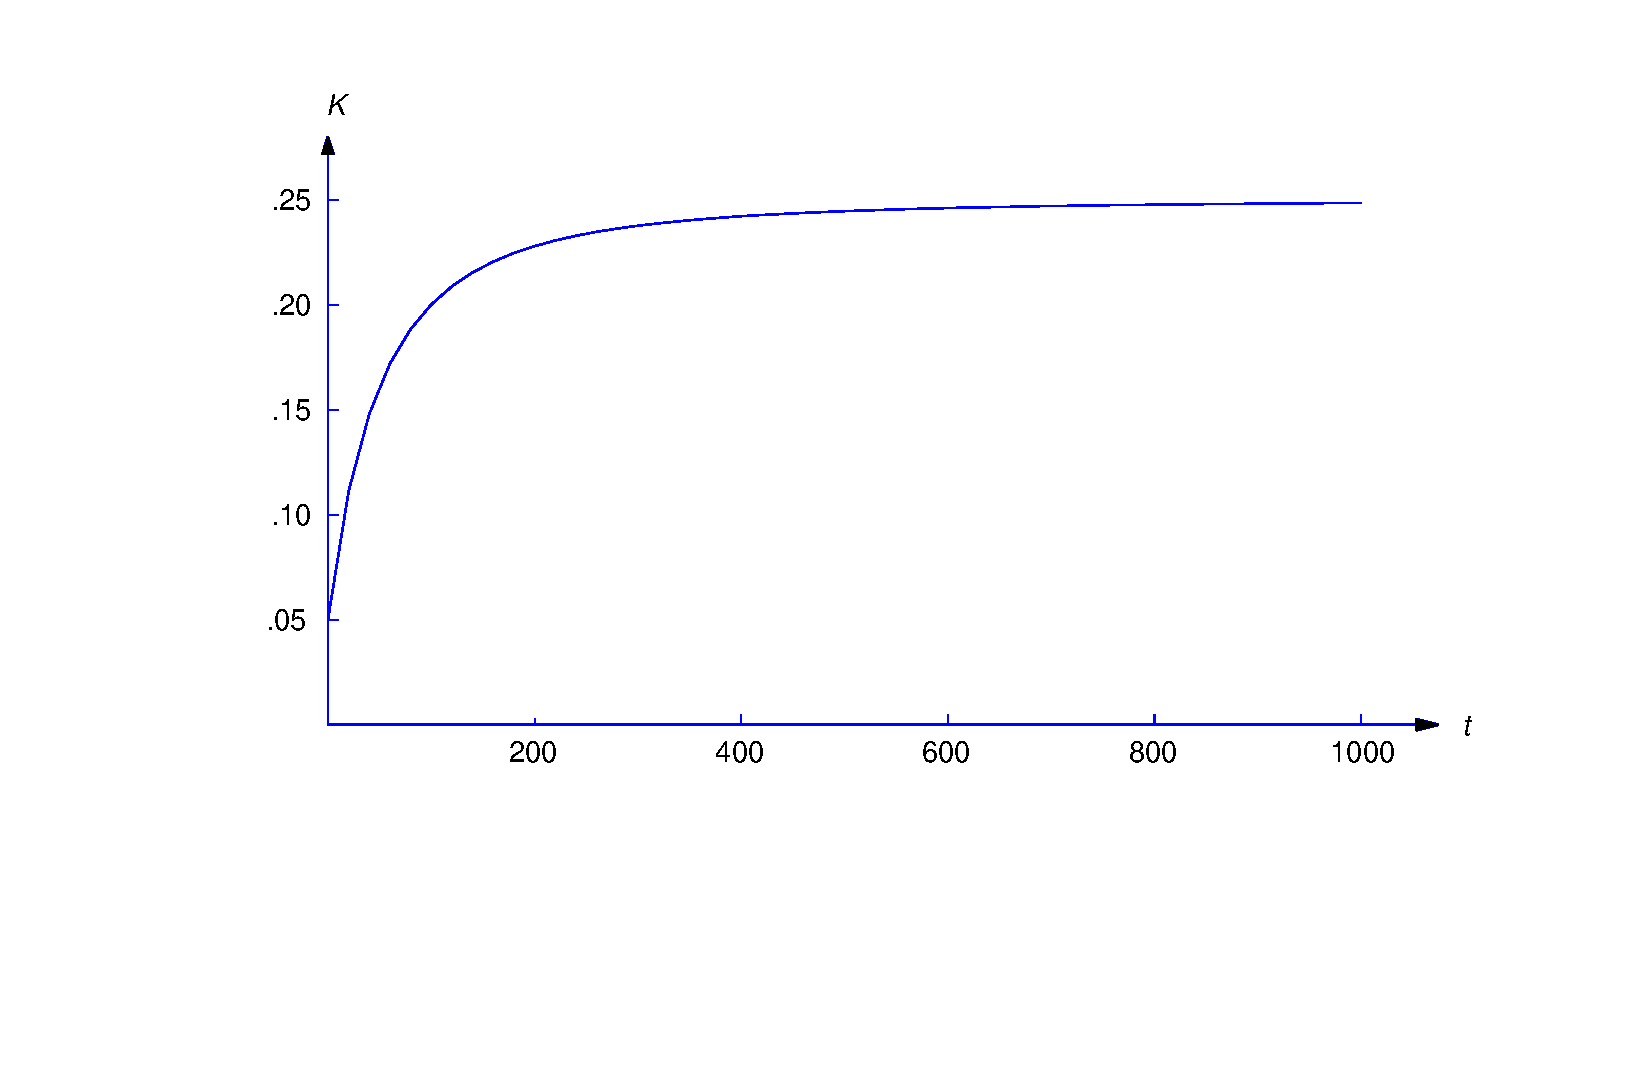
\includegraphics[bb=-78 148 689 643,width=5.67in,height=3.66in,keepaspectratio]{fig040206}
\color{blue}
  \caption{$K(t) = \dst{{1\over 4}-{2000\over(t+100)^2}}$}
  \label{figure:4.2.6}
\end{figure}

\newpage
\exercises

\begin{exerciselist}
\item\label{exer:4.2.1}
A thermometer is moved from a room where the temperature is
$70^\circ$F to a freezer where the temperature is $12^\circ
F$.  After 30 seconds the thermometer reads
$40^\circ$F.  What does it read after 2 minutes?

\item\label{exer:4.2.2}
A fluid initially at $100^\circ$C is placed outside on a
day when the temperature is $-10^\circ$C, and the
temperature of the fluid drops $20^\circ$C in one minute.
Find the temperature $T(t)$ of the fluid for $t > 0$.

\item\label{exer:4.2.3}
At 12:00 {\sc pm} a thermometer reading $10^\circ$F is placed in
a room where the temperature is $70^\circ$F.  It reads
$56^\circ$ when it's placed outside, where the temperature
is $5^\circ$F, at 12:03.  What does it read at 12:05 {\sc pm}?

\item\label{exer:4.2.4}
A thermometer initially reading $212^\circ$F is placed in a
room where the temperature is $70^\circ$F.  After 2
minutes the thermometer reads $125^\circ$F.

\begin{alist}
\item %(a)
What does the thermometer read after 4 minutes?

\item %(b)
When will the thermometer read $72^\circ$F?

\item %(c)
When will the thermometer read $69^\circ$F?
\end{alist}

\item\label{exer:4.2.5}
An object with initial temperature $150^\circ$C is placed
outside, where the temperature is $35^\circ$C.  Its
temperatures at 12:15 and 12:20 are $120^\circ$C and
$90^\circ$C, respectively.

\begin{alist}
\item %(a)
At what time was the object placed outside?

\item %(b)
When will its temperature be $40^\circ$C?
\end{alist}

\item\label{exer:4.2.6}
An object is placed in a room where the temperature is
$20^\circ$C.  The temperature of the object drops by
$5^\circ$C in 4 minutes and by $7^\circ$C in 8 minutes.
What was the temperature of the object when it was initially
placed in the room?

\item\label{exer:4.2.7}
A cup of boiling water is placed outside at 1:00 {\sc pm}.  One
minute later the temperature of the water is $152^\circ$F.
After another minute its temperature is $112^\circ$F.  What
is the outside temperature?

\item\label{exer:4.2.8}
A tank initially contains 40 gallons of pure water.  A
solution with 1 gram of salt per gallon of water is added
to the tank at 3 gal/min, and the  resulting
solution dranes out at the same rate.  Find the quantity $Q(t)$
of salt in the tank at time $t > 0$.

\item\label{exer:4.2.9}
A tank initially contains a solution of 10 pounds of salt in
60 gallons of water.  Water with 1/2 pound of salt per
gallon is added to the tank at 6 gal/min, and the
 resulting solution leaves at the same rate.
Find the quantity $Q(t)$ of salt in the tank at time
$t > 0$.

\item\label{exer:4.2.10}
A  tank initially contains 100 liters of a salt solution
with a concentration of .1 g/liter.  A solution with a
salt concentration of .3 g/liter is added to the tank at
5 liters/min, and the resulting mixture is
drained out at the same rate.  Find the concentration $K(t)$
of salt in the tank as a function of $t$.

\item\label{exer:4.2.11}
A 200 gallon tank initially contains 100 gallons of water
with 20 pounds of salt.  A salt solution with 1/4 pound of
salt per gallon is added to the tank at 4 gal/min, and the
resulting  mixture is drained out at 2 gal/min.
Find the quantity of salt in the tank as it's about to
overflow.

\item\label{exer:4.2.12}
Suppose  water is added to a tank at 10 gal/min, but leaks
out at the rate of 1/5 gal/min for each gallon in the tank.
What is the smallest capacity the tank can have if the
process is to continue indefinitely?

\item\label{exer:4.2.13}
A chemical reaction in a laboratory with volume $V$ (in ft$^3$)
produces $q_1$ ft$^3$/min of a noxious gas as a byproduct. The gas is
dangerous at concentrations greater than $\overline c$,
 but harmless at
concentrations $\le \overline c$. Intake fans at one end of the
laboratory pull in fresh air at the rate of $q_2$ ft$^3$/min and
exhaust fans at the other end exhaust the mixture of gas and air from
the
laboratory at the same rate. Assuming that the gas is always uniformly
distributed in the room and its initial concentration $c_0$ is at a
safe level, find the smallest value of $q_2$ required to maintain safe
conditions in the laboratory for all time.

\item\label{exer:4.2.14}
A 1200-gallon tank initially contains 40 pounds of salt
dissolved in 600 gallons of water.  Starting at $t_0=0$,
water that contains 1/2 pound of salt per gallon is added to
the tank at the rate of 6 gal/min and the
resulting mixture  is drained from the tank at 4 gal/min.  Find the
quantity $Q(t)$ of salt in the tank at any time $t > 0$
prior to overflow.

\item\label{exer:4.2.15}
Tank $T_1$  initially contain 50 gallons of pure water. Starting at
$t_0=0$,  water that contains 1 pound of salt per gallon is poured into
$T_1$ at  the rate of  2 gal/min.
The  mixture is drained from
$T_1$ at the same rate into a second tank $T_2$, which initially
contains  50 gallons of pure water.  Also starting at
$t_0=0$, a mixture from another source that contains 2  pounds of salt
per gallon is poured
into $T_2$  at the rate of 2 gal/min.  The  mixture is drained
from $T_2$ at the rate of 4 gal/min.

\begin{alist}
\item % (a)
 Find a differential
equation for the quantity $Q(t)$ of salt in  tank $T_2$ at time $t > 0$.
\item % (b)
Solve the equation derived  in \part{a} to determine $Q(t)$.
\item % (c)
 Find $\lim_{t\to\infty}Q(t)$.
\end{alist}

\item\label{exer:4.2.16}
Suppose an object  with initial temperature $T_0$
is placed in a sealed container, which is in turn placed in a medium with
temperature $T_m$. Let the initial
temperature of the container be $S_0$. Assume that the temperature of the
object does not affect the temperature of the container, which in turn does
not affect the temperature of the medium. (These assumptions  are
reasonable, for example, if the object is a cup of coffee, the container is
a house, and the medium is the atmosphere.)

\begin{alist}
\item % (a)
Assuming that the container and the medium have distinct temperature
decay constants $k$ and $k_m$ respectively, use Newton's law of
cooling to find the temperatures $S(t)$ and $T(t)$ of the container
and object at time $t$.

\item % (b)
Assuming that the container and the medium have the same temperature
decay constant $k$, use Newton's law of cooling to find the
temperatures $S(t)$ and $T(t)$ of the container and object at time
$t$.

\item % (c)
Find $\lim._{t\to\infty}S(t)$  and $\lim_{t\to\infty}T(t)$ .
\end{alist}

\item\label{exer:4.2.17}  %\exercisemolten
In  our previous examples and exercises concerning Newton's law of cooling
we assumed that
the temperature of the medium remains constant.  This model is adequate
if the heat lost or gained by the object is
insignificant compared to the heat required to cause an appreciable change
in the temperature of the medium. If this isn't  so,  we
must use a model that accounts for the heat exchanged between the object
and the medium. Let $T=T(t)$ and $T_m=T_m(t)$  be the temperatures of the
object and the medium, respectively, and let $T_0$  and $T_{m0}$ be
their
initial values.  Again, we assume that $T$  and $T_m$ are related by
Newton's law of cooling,
$$
T'=-k(T-T_m).
\eqno{\rm (A)}
$$
We also assume that the change in heat of the object as its
temperature changes from $T_0$ to $T$  is $a(T-T_0)$
and that the change in heat of the medium  as its
temperature changes from $T_{m0}$ to $T_m$  is $a_m(T_m-T_{m0})$,
where $a$
and $a_m$ are positive constants  depending  upon the masses and
thermal properties of the
object and medium, respectively.  If we assume that the total heat of
the system consisting of the object and the medium remains constant
(that is, energy is conserved), then
$$
a(T-T_0)+a_m(T_m-T_{m0})=0.
\eqno{\rm (B)}
$$

\begin{alist}
\item % (a)
Equation (A) involves  two unknown functions $T$ and $T_m$.
 Use (A) and (B) to derive a
differential equation involving only $T$.
\item % (b)
Find $T(t)$ and $T_m(t)$ for $t>0$.
\item % (c)
Find $\lim_{t\to\infty}T(t)$ and
 $\lim_{t\to\infty}T_m(t)$.
\end{alist}

\item\label{exer:4.2.18} Control mechanisms allow fluid to flow into a tank
at a rate proportional to the volume $V$ of fluid in the tank, and to
flow
out at a rate proportional to $V^2$. Suppose $V(0)=V_0$ and the
constants of proportionality are $a$ and $b$, respectively.
Find $V(t)$  for $t>0$ and find $\lim_{t\to\infty}V(t)$.

\item\label{exer:4.2.19}
Identical tanks $T_1$ and $T_2$ initially contain $W$ gallons each of
pure water. Starting at $t_0=0$, a salt solution with constant
concentration $c$ is pumped into $T_1$ at $r$ gal/min and drained from
$T_1$ into $T_2$ at the same rate. The resulting mixture in $T_2$ is
also drained at the same rate. Find the concentrations $c_1(t)$
and $c_2(t)$ in tanks $T_1$ and $T_2$ for $t>0$.

\item\label{exer:4.2.20}
An infinite sequence of identical tanks $T_1$, $T_2$, \dots, $T_n$, \dots,
initially contain $W$ gallons
each of pure water.  They are hooked together so that fluid drains
from $T_n$ into  $T_{n+1}\,(n=1,2,\cdots)$.
A salt solution is circulated through the tanks so that it enters and
leaves each tank at the constant rate of $r$ gal/min.
The solution has a concentration of
$c$  pounds of salt per
gallon when it enters $T_1$.

\begin{alist}
\item % (a)
Find the concentration $c_n(t)$
in tank $T_n$ for $t>0$.
\item % (b)
  Find $\lim_{t\to\infty}c_n(t)$ for each $n$.
\end{alist}

\item\label{exer:4.2.21}
Tanks $T_1$  and $T_2$ have capacities $W_1$ and $W_2$ liters,
respectively.
Initially they are both full of dye solutions with concentrations $c_{1}$
and $c_2$ grams per liter. Starting at $t_0=0$,  the solution from $T_1$
is pumped into $T_2$ at a rate of $r$  liters per minute,
and the solution from $T_2$
is pumped into $T_1$ at the same rate.

\begin{alist}
\item % (a)
Find the concentrations $c_1(t)$ and $c_2(t)$ of the dye in $T_1$
and $T_2$ for $t>0$.
\item % (b)
Find $\lim_{t\to\infty}c_1(t)$  and $\lim_{t\to\infty}c_2(t)$.
\end{alist}

\item\label{exer:4.2.22} \Lex
Consider the mixing problem of Example~\ref{example:4.2.3}, but without
the assumption that the mixture is stirred instantly so that the salt
is always uniformly distributed throughout the mixture. Assume instead
that the distribution approaches uniformity as $t\to\infty$.
In this case the differential equation for $Q$ is  of the form
$$
Q'+{a(t)\over150}Q=2
$$
where  $\lim_{t\to\infty}a(t)=1$.
\begin{alist}
\item % (a)
Assuming that
$Q(0)=Q_0$, can you guess the value of
$\lim_{t\to\infty}Q(t)$?.
\item % (b)
Use numerical methods to  confirm  your guess in the these cases:
$$
\mbox{\part{i}\;   }  a(t)=t/(1+t)  \mbox{\quad    \part{ii}\;  }
a(t)=1-e^{-t^2}  \mbox{\quad    \part{iii}\;  }
 a(t)=1-\sin(e^{-t}).
$$
\end{alist}

\item\label{exer:4.2.23} \Lex
Consider the mixing problem of Example~\ref{example:4.2.4} in a tank with
infinite capacity, but without the assumption that the mixture is
stirred instantly so that the salt is always uniformly distributed
throughout the mixture. Assume instead that the distribution
approaches uniformity as $t\to\infty$. In this case the differential
equation for $Q$ is of the form
$$
Q'+{a(t)\over t+100}Q=1
$$
where  $\lim_{t\to\infty}a(t)=1$.
\begin{alist}
\item % (a)
Let $K(t)$ be the concentration of salt at time $t$. Assuming that
$Q(0)=Q_0$, can you guess the value of $\lim_{t\to\infty}K(t)$?
\item % (b)
Use numerical methods to  confirm  your guess in the these cases:
$$
\mbox{\part{i}\;  }  a(t)=t/(1+t)\; \mbox{\;   \part{ii}\;   }
a(t)=1-e^{-t^2}  \mbox{\;   \part{iii}\;   }
 a(t)=1+\sin(e^{-t}).
$$
\end{alist}

\end{exerciselist}
